\appendix
\section{Appendix} \label{Appendix}


Here, we provide further details that are not discussed in the main paper and include extra experimental results. The appendix is structured as follows:

\startcontents[appendices]
\printcontents[appendices]{l}{1}{\setcounter{tocdepth}{3}}

\subsection{Pseudocode} \label{pseudpcode}
Algorithm~\ref{alg_rc} and Algorithm~\ref{alg_plc} present the pseudocode for \textbf{residual compensation} and \textbf{partial-layer compression}, respectively.
Algorithm~\ref{alg_plc} identifies the optimal number of last layers $k$ to compress, along with their corresponding layer compression ratio $R_l$.
Specifically, for a model with $N$ layers, we iterate over candidate values of $k'$ using a step size $s$ and compute the associated $R_l'$ for each.
For each candidate configuration, we invoke Algorithm~\ref{alg_rc} to perform the compression, after which we compute the final-layer error relative to the original model.
The configuration yielding the lowest final-layer error is selected as the optimal compression setting.

\begin{algorithm}[ht]
    \caption{Pseudocode of Residual Compensation}
    \label{alg_rc}
    \renewcommand{\algorithmicrequire}{\textbf{Input:}}
    \renewcommand{\algorithmicensure}{\textbf{Output:}}
    
    \begin{algorithmic}[1]
        \REQUIRE Original LLM: $M$, weight matrix: $\boldsymbol{W}_i\in\mathbb{R}^{m\times n}$, layer compression ratio: $R_l$, residual compensation rank: $r_r$   %%input
        \ENSURE Compressed weight matrix set $\mathrm{Set}_{\boldsymbol{W'}}(i)$ of layer $i$     %%output
        
        \STATE $CD \gets$ Randomly collect calibration samples from the dataset
        

        \STATE $\mathrm{Set}_{\boldsymbol{S}} \gets$ \textsc{Whitening}($M$, $CD$), $\mathrm{Set}_{\boldsymbol{W'}}(i) \gets \emptyset$ \hfill $\triangleright$ Initialize sets of weight matrices

        \STATE $r = (1-R_l)(m \cdot n)/(m+n) $, $r_i = r-r_r$ \hfill $\triangleright$ Calculate the intermediate rank
            
        \STATE $\boldsymbol{S}_i \gets \mathrm{Set}_{\boldsymbol{S}}(i)$ \hfill $\triangleright$ Extract scaling matrices of current weight matrices

        \STATE $\boldsymbol{U}_{i,r_i}$, $\boldsymbol{\Sigma}_{i,r_i}$, $\boldsymbol{V}_{i,r_i}^T$ $\gets$ $\boldsymbol{W}_{i,r_i}\boldsymbol{S}_i^{-1}$ $\gets$ \textsc{SVD\_Trunc}($\boldsymbol{W}_i\boldsymbol{S}_i$)$\boldsymbol{S}_i^{-1}$ \hfill $\triangleright$ SVD truncation on weight matrices

        \STATE $\boldsymbol{R}_{i}$ $\gets$ \textsc{Cal\_Res}($\boldsymbol{W}_i$, $\boldsymbol{W}_{i,r_i}$) \hfill $\triangleright$ Calculate residual matrices

        \STATE $\boldsymbol{U}_{i,r_r}$, $\boldsymbol{\Sigma}_{i,r_r}$, $\boldsymbol{V}_{i,r_r}^T$ $\gets$ $\boldsymbol{R}_{i,r_r}$ $\gets$ \textsc{SVD\_Trunc}($\boldsymbol{R}_i$) \hfill $\triangleright$ SVD truncation on residual matrices

        \STATE $\hat{\boldsymbol{U}}_{i,r_r}$ $\gets$ \textsc{Mul}($\boldsymbol{U}_{i,r_r}$, $\sqrt{\boldsymbol{\Sigma}_{i,r_r}}$), $\hat{\boldsymbol{V}}_{i,r_r}$ $\gets$ \textsc{Mul}($\sqrt{\boldsymbol{\Sigma}_{i,r_r}}$, $\boldsymbol{V}_{i,r_r}^T$) \hfill $\triangleright$ Absorb singular values

        \STATE $\hat{\boldsymbol{U}}_{i,r_i}$ $\gets$ \textsc{Mul}($\boldsymbol{U}_{i,r_i}$, $\sqrt{\boldsymbol{\Sigma}_{i,r_i}}$), $\hat{\boldsymbol{V}}_{i,r_i}$ $\gets$ \textsc{Mul}($\sqrt{\boldsymbol{\Sigma}_{i,r_i}}$, $\boldsymbol{V}_{i,r_i}^T$) 
                
        \STATE $\hat{\boldsymbol{U}}_{i,r}$ $\gets$ \textsc{Comb}($\hat{\boldsymbol{U}}_{i,r_r}$, $\hat{\boldsymbol{U}}_{i,r_i}$), $\hat{\boldsymbol{V}}_{i,r}$ $\gets$ \textsc{Comb}($\hat{\boldsymbol{V}}_{i,r_r}$, $\hat{\boldsymbol{V}}_{i,r_i}$) \hfill $\triangleright$ Combine weight matrices  

        \STATE $\mathrm{Set}_{\boldsymbol{W'}}(i)$ $\gets$ ($\hat{\boldsymbol{U}}_{i,r}$, $\hat{\boldsymbol{V}}_{i,r}$) $\cup$ $\mathrm{Set}_{\boldsymbol{W'}}(i)$ \hfill $\triangleright$ Append decomposed weight matrices
            
        
        \RETURN $\mathrm{Set}_{\boldsymbol{W'}}(i)$
    \end{algorithmic}
\end{algorithm}

\begin{algorithm}[ht]
  \caption{Pseudocode of Partial-layer Compression}
    \label{alg_plc}
    \renewcommand{\algorithmicrequire}{\textbf{Input:}}
    \renewcommand{\algorithmicensure}{\textbf{Output:}}
  %
  \begin{algorithmic}[1]
    \REQUIRE Original LLM: $M$, number of model layers: $N$, overall compression ratio: $R_o$, step: $s$ %%input
    \ENSURE Number of layers to compress: $k$, layer compression ratio: $R_l$   %%output

    \STATE $CD \gets$ Randomly collect calibration samples from the dataset
    
    \STATE $\mathrm{Set}_{\boldsymbol{W}} \gets M$ \hfill $\triangleright$ Extract the set of weight matrices in $M$
    
    \STATE $\mathrm{Set}_{k'} \gets \{\,k' \mid k'=s,2s,\dots,N-s\}$ \hfill $\triangleright$ Obtain candidate compressed layer numbers
    %
    \STATE $ Lowest\_Err \gets +\infty$
    %
    \FOR{each $k'$ in $\mathrm{Set}_{k'}$}
        \STATE $R_l' \gets (N \cdot R_o) / k'$ \hfill $\triangleright$ Calculate corresponding layer compression ratio 
        \IF{$R_l' \ge 0$}
            %
            \STATE $M_{TMP} \gets$ \textsc{Deep\_Copy}$(M)$
            %
            \FOR{$i \in [N-k'+1, N]$}
                \STATE $\textbf{W}_i \gets$ $\mathrm{Set}_{\boldsymbol{W}}(i)$ \hfill $\triangleright$ Initialize weight matrices to compress
                \STATE $\mathrm{Set}_{\boldsymbol{W'}}(i) \gets$ \textsc{Residual Compensation}($M$, $\textbf{W}_i$, $R_l'$, $r_r$)
                \STATE Replace weights of layer $i$ in $M_{TMP}$ with $\mathrm{Set}_{\boldsymbol{W'}}(i)$
            \ENDFOR
            %
            \STATE $Err \gets$ \textsc{Cal\_Error}($M, M_{TMP}, CD, Layer(N)$) \hfill $\triangleright$ Calculate the last layer output error
            \IF{$Err < Lowest\_Err$} 
                \STATE $Lowest\_Err \gets Err$ \hfill $\triangleright$ Search for the lowest layer-wise error
                \STATE $k   \gets k'$
                \STATE $R_l \gets R_l'$
            \ENDIF
        \ENDIF
    \ENDFOR
    %
    \RETURN $k, R_l$
  \end{algorithmic}
\end{algorithm}

\subsection{Layer-wise Error Comparison}
As discussed in Section~\ref{sec_plc}, the same observation also holds here. We conduct experiments on Mistral-7B~\cite{jiang2023mistral} and Vicuna-7B~\cite{chiang2023vicuna}, and the results are presented in Figure~\ref{layer-wise_error_comparison_llm-1}.

\begin{figure}[ht]
  \centering

  \begin{subfigure}[t]{0.49\linewidth}
    \centering
    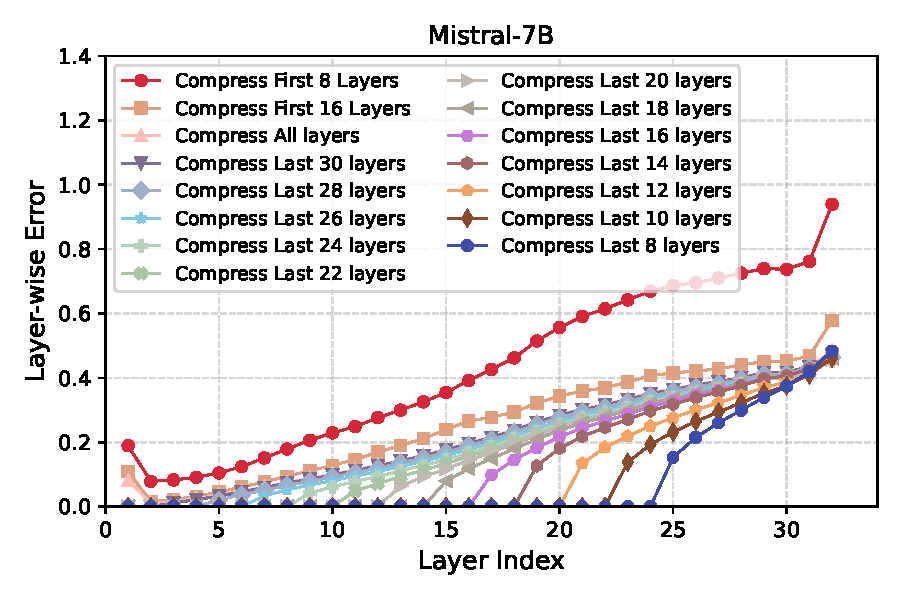
\includegraphics[width=\linewidth]{CPAL-2025-template/a_figures/mistral_loss_comparison.pdf}
  \end{subfigure}
  \begin{subfigure}[t]{0.49\linewidth}
    \centering
    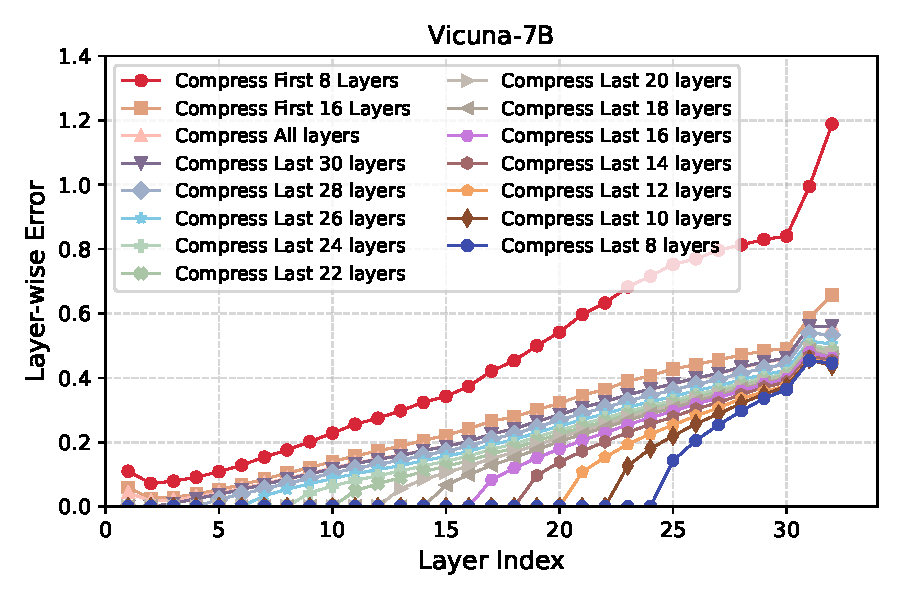
\includegraphics[width=\linewidth]{CPAL-2025-template/a_figures/vicuna_loss_comparison.pdf}
  \end{subfigure}

  \caption{
    Layer-wise error comparison between the original model, Mistral-7B, and Vicuna-7B compressed by ERC-SVD with different layer selection strategies on WikiText-2. The overall compression ratio is 20\%, and all layer selection strategies strictly adhere to the compression constraint.
  }
  \label{layer-wise_error_comparison_llm-1}
\end{figure}

\subsection{Additional Results}
In this section, we present additional results from four perspectives: Section~\ref{more_results_on_large} reports zero-shot accuracy on larger-scale LLMs, Section~\ref{more_results_on_multiple} reports zero-shot accuracy across multiple LLM families, Section~\ref{ablation_study_50_60} presents ablation results under compression ratios 40\%, 50\%, and 60\%, and Section~\ref{calibration-data} demonstrates the impact of calibration data.

\subsubsection{Results on Larger-scale LLMs} \label{more_results_on_large}
In Table~\ref{larger-llm-acc}, we present zero-shot accuracy results for LLaMA-13B~\cite{touvron2023llama}, LLaMA-30B~\cite{touvron2023llama}, LLaMA-2-13B~\cite{touvron2023llama2}, OPT-13B~\cite{zhang2022opt}, and OPT-30B~\cite{zhang2022opt}. Across these evaluation datasets, ERC-SVD consistently outperforms SVD-LLM, with only one minor exception.
\begin{table}[t]
\centering
\caption{Zero-shot accuracy results across larger-scale LLMs under 20\% compression ratio.}
\label{larger-llm-acc}
% \vspace{1mm}
% \vspace{-5pt}
\small
\resizebox{\textwidth}{!}{
\begin{tabular}{c|c|cccccccc}
    \toprule
     \textsc{Model} & \textsc{Method} & Openb.$\uparrow$  & ARC\_e$\uparrow$ & WinoG.$\uparrow$ & HellaS.$\uparrow$ & ARC\_c$\uparrow$ & PIQA$\uparrow$ & MathQA$\uparrow$ & Average\textcolor{green!60!black}{$\uparrow$}\\
    \midrule
        \multirow{2}{*}{LLaMA-13B}
              
                               & \cellcolor{white} SVD-LLM & \cellcolor{white} 0.27 & \cellcolor{white} 0.62 & \cellcolor{white} 0.66 & \cellcolor{white} 0.46 & \cellcolor{white} 0.33 & \cellcolor{white} 0.72 & \cellcolor{white} 0.26 & \cellcolor{white} 0.47 \\
        \cmidrule{2-10}
                               & \cellcolor{cyan!10} \textbf{ERC-SVD} & \cellcolor{cyan!10} \textbf{0.28} & \cellcolor{cyan!10} \textbf{0.69} & \cellcolor{cyan!10} \textbf{0.69} & \cellcolor{cyan!10} \textbf{0.54} & \cellcolor{cyan!10} \textbf{0.39} & \cellcolor{cyan!10} \textbf{0.75} & \cellcolor{cyan!10} \textbf{0.26} & \cellcolor{cyan!10} \textbf{0.52} \\

    \midrule
        \multirow{2}{*}{LLaMA-30B}
              
                              & \cellcolor{white} SVD-LLM & \cellcolor{white} 0.29 & \cellcolor{white} 0.72 & \cellcolor{white} 0.73 & \cellcolor{white} 0.51 & \cellcolor{white} 0.38 & \cellcolor{white} 0.74 & \cellcolor{white} 0.27 & \cellcolor{white} 0.51 \\
        \cmidrule{2-10}
                               & \cellcolor{cyan!10} \textbf{ERC-SVD} & \cellcolor{cyan!10} \textbf{0.30} & \cellcolor{cyan!10} \textbf{0.73} & \cellcolor{cyan!10} \textbf{0.73} & \cellcolor{cyan!10} \textbf{0.59} & \cellcolor{cyan!10} \textbf{0.43} & \cellcolor{cyan!10} \textbf{0.78} & \cellcolor{cyan!10} \textbf{0.29} & \cellcolor{cyan!10} \textbf{0.55} \\
    \midrule
        \multirow{2}{*}{LLaMA-2-13B}
              
                              & \cellcolor{white} SVD-LLM & \cellcolor{white} 0.27 & \cellcolor{white} 0.63 & \cellcolor{white} 0.66 & \cellcolor{white} 0.44 & \cellcolor{white} 0.31 & \cellcolor{white} 0.71 & \cellcolor{white} 0.26 & \cellcolor{white} 0.47 \\
        \cmidrule{2-10}
                               & \cellcolor{cyan!10} \textbf{ERC-SVD} & \cellcolor{cyan!10} \textbf{0.31} & \cellcolor{cyan!10} \textbf{0.67} & \cellcolor{cyan!10} \textbf{0.68} & \cellcolor{cyan!10} \textbf{0.47} & \cellcolor{cyan!10} \textbf{0.38} & \cellcolor{cyan!10} \textbf{0.74} & \cellcolor{cyan!10} \textbf{0.27} & \cellcolor{cyan!10} \textbf{0.50} \\

    \midrule
        \multirow{2}{*}{OPT-13B}
              
                              & \cellcolor{white} SVD-LLM & \cellcolor{white} 0.24 & \cellcolor{white} 0.62 & \cellcolor{white} 0.64 & \cellcolor{white} \textbf{0.47} & \cellcolor{white} 0.30 & \cellcolor{white} 0.72 & \cellcolor{white} 0.24 & \cellcolor{white} 0.46 \\
        \cmidrule{2-10}
                               & \cellcolor{cyan!10} \textbf{ERC-SVD} & \cellcolor{cyan!10} \textbf{0.24} & \cellcolor{cyan!10} \textbf{0.63} & \cellcolor{cyan!10} \textbf{0.65} & \cellcolor{cyan!10} 0.45 & \cellcolor{cyan!10} \textbf{0.30} & \cellcolor{cyan!10} \textbf{0.73} & \cellcolor{cyan!10} \textbf{0.24} & \cellcolor{cyan!10} \textbf{0.46} \\

    \midrule
        \multirow{2}{*}{OPT-30B}
              
                              & \cellcolor{white} SVD-LLM & \cellcolor{white} \textbf{0.29} & \cellcolor{white} 0.67 & \cellcolor{white} 0.65 & \cellcolor{white} \textbf{0.51} & \cellcolor{white} 0.33 & \cellcolor{white} 0.75 & \cellcolor{white} 0.25 & \cellcolor{white} 0.49 \\
        \cmidrule{2-10}
                               & \cellcolor{cyan!10} \textbf{ERC-SVD} & \cellcolor{cyan!10} 0.28 & \cellcolor{cyan!10} \textbf{0.68} & \cellcolor{cyan!10} \textbf{0.67} & \cellcolor{cyan!10} 0.50 & \cellcolor{cyan!10} \textbf{0.34} & \cellcolor{cyan!10} \textbf{0.76} & \cellcolor{cyan!10} \textbf{0.25} & \cellcolor{cyan!10} \textbf{0.49} \\
    \bottomrule
\end{tabular}
}
\end{table}

\subsubsection{Results on Multiple LLM Families} \label{more_results_on_multiple}
We also evaluate the zero-shot accuracy of OPT-6.7B~\cite{zhang2022opt}, Mistral-7B~\cite{jiang2023mistral}, and Vicuna-7B~\cite{chiang2023vicuna}. Results are shown in Table~\ref{multiple-llm-acc}, and our method consistently outperforms SVD-LLM across these diverse LLM architectures.
In addition, we conduct experiments on Qwen-3-8B~\cite{yang2025qwen3}, with perplexity and zero-shot accuracy results reported in Table~\ref{new-model-acc}.

\begin{table}[t]
\centering
\caption{Performance of Qwen-3-8B under 20\% to 60\% compression ratios (``\textsc{Ratio}'').}
\label{new-model-acc}
% \vspace{1mm}
% \vspace{-5pt}
\small
\resizebox{\textwidth}{!}{
\begin{tabular}{c|c|ccc|cccccccc}
    \toprule
     \textsc{Ratio} & \textsc{Method} & WikiText-2\textcolor{blue}{$\downarrow$} & PTB\textcolor{blue}{$\downarrow$} & C4\textcolor{blue}{$\downarrow$} & Openb.$\uparrow$  & ARC\_e$\uparrow$ & WinoG.$\uparrow$ & HellaS.$\uparrow$ & ARC\_c$\uparrow$ & PIQA$\uparrow$ & MathQA$\uparrow$ & Average\textcolor{green!60!black}{$\uparrow$}\\
    \midrule
                               & \cellcolor{white} \textcolor{gray}{Original} & \cellcolor{white} \textcolor{gray}{9.71} & \cellcolor{white} \textcolor{gray}{15.43} & \cellcolor{white} \textcolor{gray}{15.52} & \cellcolor{white} \textcolor{gray}{0.31} & \cellcolor{white} \textcolor{gray}{0.83} & \cellcolor{white} \textcolor{gray}{0.68} & \cellcolor{white} \textcolor{gray}{0.57} & \cellcolor{white} \textcolor{gray}{0.56} & \cellcolor{white} \textcolor{gray}{0.77} & \cellcolor{white} \textcolor{gray}{0.49} & \cellcolor{white} \textcolor{gray}{0.60}\\   
    \midrule
    \multirow{2}{*}{20\%}
                               & \cellcolor{white} SVD-LLM & \cellcolor{white} 37.52 & \cellcolor{white} \textbf{40.73} & \cellcolor{white} 47.25 & \cellcolor{white} \textbf{0.20} & \cellcolor{white} 0.50 & \cellcolor{white} 0.55 & \cellcolor{white} 0.35 & \cellcolor{white} 0.24 & \cellcolor{white} 0.64 & \cellcolor{white} 0.22 & \cellcolor{white} 0.39 \\
                               
                               & \cellcolor{cyan!10} \textbf{ERC-SVD} & \cellcolor{cyan!10} \textbf{35.11} & \cellcolor{cyan!10} 42.77 & \cellcolor{cyan!10} \textbf{43.10} & \cellcolor{cyan!10} 0.19 & \cellcolor{cyan!10} \textbf{0.54} & \cellcolor{cyan!10} \textbf{0.58} & \cellcolor{cyan!10} \textbf{0.35} & \cellcolor{cyan!10} \textbf{0.25} & \cellcolor{cyan!10} \textbf{0.66} & \cellcolor{cyan!10} \textbf{0.24} & \cellcolor{cyan!10} \textbf{0.40} \\
    \midrule
    \multirow{2}{*}{30\%}
                               & \cellcolor{white} SVD-LLM & \cellcolor{white} 72.33 & \cellcolor{white} 67.68 & \cellcolor{white} 86.56 & \cellcolor{white} 0.15 & \cellcolor{white} \textbf{0.42} & \cellcolor{white} 0.53 & \cellcolor{white} 0.30 & \cellcolor{white} 0.19 & \cellcolor{white} 0.60 & \cellcolor{white} 0.21 & \cellcolor{white} 0.34 \\
                               
                               & \cellcolor{cyan!10} \textbf{ERC-SVD} & \cellcolor{cyan!10} \textbf{66.89} & \cellcolor{cyan!10} \textbf{71.48} & \cellcolor{cyan!10} \textbf{82.28} & \cellcolor{cyan!10} \textbf{0.16} & \cellcolor{cyan!10} 0.41 & \cellcolor{cyan!10} \textbf{0.53} & \cellcolor{cyan!10} \textbf{0.30} & \cellcolor{cyan!10} \textbf{0.20} & \cellcolor{cyan!10} \textbf{0.61} & \cellcolor{cyan!10} \textbf{0.22} & \cellcolor{cyan!10} \textbf{0.35} \\
    \midrule
    \multirow{2}{*}{40\%}
                               & \cellcolor{white} SVD-LLM & \cellcolor{white} 143.28 & \cellcolor{white} 122.55 & \cellcolor{white} 162.99 & \cellcolor{white} 0.12 & \cellcolor{white} 0.34 & \cellcolor{white} 0.51 & \cellcolor{white} 0.28 & \cellcolor{white} 0.16 & \cellcolor{white} \textbf{0.58} & \cellcolor{white} 0.22 & \cellcolor{white} 0.32 \\
                               
                               & \cellcolor{cyan!10} \textbf{ERC-SVD} & \cellcolor{cyan!10} \textbf{135.66} & \cellcolor{cyan!10} \textbf{113.34} & \cellcolor{cyan!10} \textbf{154.32} & \cellcolor{cyan!10} \textbf{0.12} & \cellcolor{cyan!10} \textbf{0.35} & \cellcolor{cyan!10} \textbf{0.52} & \cellcolor{cyan!10} \textbf{0.29} & \cellcolor{cyan!10} \textbf{0.17} & \cellcolor{cyan!10} 0.57 & \cellcolor{cyan!10} \textbf{0.22} & \cellcolor{cyan!10} \textbf{0.32} \\
    \midrule
    \multirow{2}{*}{50\%}
                               & \cellcolor{white} SVD-LLM & \cellcolor{white} 274.04 & \cellcolor{white} 226.30 & \cellcolor{white} 308.11 & \cellcolor{white} 0.12 & \cellcolor{white} 0.30 & \cellcolor{white} 0.50 & \cellcolor{white} 0.27 & \cellcolor{white} 0.18 & \cellcolor{white} 0.55 & \cellcolor{white} 0.20 & \cellcolor{white} 0.30 \\
                               
                               & \cellcolor{cyan!10} \textbf{ERC-SVD} & \cellcolor{cyan!10} \textbf{247.57} & \cellcolor{cyan!10} \textbf{170.82} & \cellcolor{cyan!10} \textbf{294.00} & \cellcolor{cyan!10} \textbf{0.12} & \cellcolor{cyan!10} \textbf{0.30} & \cellcolor{cyan!10} \textbf{0.50} & \cellcolor{cyan!10} \textbf{0.28} & \cellcolor{cyan!10} \textbf{0.18} & \cellcolor{cyan!10} \textbf{0.56} & \cellcolor{cyan!10} \textbf{0.22} & \cellcolor{cyan!10} \textbf{0.31} \\
    \midrule
    \multirow{2}{*}{60\%}
                               & \cellcolor{white} SVD-LLM & \cellcolor{white} 462.53 & \cellcolor{white} 338.39 & \cellcolor{white} 528.22 & \cellcolor{white} 0.11 & \cellcolor{white} 0.27 & \cellcolor{white} \textbf{0.48} & \cellcolor{white} 0.26 & \cellcolor{white} 0.18 & \cellcolor{white} \textbf{0.54} & \cellcolor{white} 0.20 & \cellcolor{white} 0.29 \\
                               
                               & \cellcolor{cyan!10} \textbf{ERC-SVD} & \cellcolor{cyan!10} \textbf{460.73} & \cellcolor{cyan!10} \textbf{287.19} & \cellcolor{cyan!10} \textbf{522.29} & \cellcolor{cyan!10} \textbf{0.11} & \cellcolor{cyan!10} \textbf{0.27} & \cellcolor{cyan!10} 0.46 & \cellcolor{cyan!10} \textbf{0.27} & \cellcolor{cyan!10} \textbf{0.19} & \cellcolor{cyan!10} 0.53 & \cellcolor{cyan!10} \textbf{0.20} & \cellcolor{cyan!10} \textbf{0.29} \\

    \bottomrule
\end{tabular}
}
\end{table}

\subsubsection{Additional Ablation Results} \label{ablation_study_50_60}
The ablation results for LLaMA-2-7B~\cite{touvron2023llama2} under 40\%, 50\%, and 60\% compression ratios are presented in Table~\ref{more_ablation_study}.
A similar trend can also be observed here: incorporating both REC and PLC leads to a substantial reduction in perplexity across all settings.

\begin{table}[ht]
\centering
\caption{Ablation results of residual compensation and partial-layer compression on LLaMA-2-7B~\cite{touvron2023llama2} under 40\%, 50\%, and 60\% compression ratios.}
\label{more_ablation_study}
% \vspace{1mm}
% \vspace{-5pt}
\small
\resizebox{\textwidth}{!}{
\begin{tabular}{c|c|cc|c|cccccccc}
    \toprule
     \textsc{Ratio} & \textsc{Method} & REC & PLC & C4\textcolor{blue}{$\downarrow$} & Openb.$\uparrow$  & ARC\_e$\uparrow$ & WinoG.$\uparrow$ & HellaS.$\uparrow$ & ARC\_c$\uparrow$ & PIQA$\uparrow$ & MathQA$\uparrow$ & Average\textcolor{green!60!black}{$\uparrow$}\\

     \midrule
        \multirow{5}{*}{40\%}  
                               & ASVD & \cellcolor{white} - & \cellcolor{white} - & \cellcolor{white} NaN & \cellcolor{white} 0.15 & \cellcolor{white} 0.25 & \cellcolor{white} 0.50 & \cellcolor{white} 0.26 & \cellcolor{white} 0.22 & \cellcolor{white} 0.52 & \cellcolor{white} 0.18 & \cellcolor{white} 0.30\\
        
                               & SVD-LLM & \cellcolor{white} - & \cellcolor{white} - & \cellcolor{white} 61.96 & \cellcolor{white} 0.16 & \cellcolor{white} 0.35 & \cellcolor{white} 0.55 & \cellcolor{white} 0.30 & \cellcolor{white} 0.20 & \cellcolor{white} 0.57 & \cellcolor{white} 0.23 & \cellcolor{white} 0.34\\

        \cmidrule{2-13}
        & \multirow{3}{*}{\textbf{ERC-SVD}}
                               & \ding{51} & \ding{55} & 54.19 & 0.17 & 0.37 & 0.54 & 0.32 & 0.21 & 0.57 & 0.23 & 0.34\\

                               & & \ding{55} & \ding{51} & 45.13 & 0.18 & 0.40 & 0.55 & 0.33 & 0.24 & 0.61 & 0.21 & 0.36\\

                               & & \cellcolor{cyan!10} \ding{51} & \cellcolor{cyan!10} \ding{51} & \cellcolor{cyan!10} \textbf{43.19}  & \cellcolor{cyan!10} 0.20 & \cellcolor{cyan!10} 0.43 & \cellcolor{cyan!10} 0.57 & \cellcolor{cyan!10} 0.35 & \cellcolor{cyan!10} 0.24 & \cellcolor{cyan!10} 0.63 & \cellcolor{cyan!10} 0.23 & \cellcolor{cyan!10} \textbf{0.38} \\
                               
    \midrule
        \multirow{5}{*}{50\%}  
                               & ASVD & \cellcolor{white} - & \cellcolor{white} - & \cellcolor{white} NaN & \cellcolor{white} 0.13 & \cellcolor{white} 0.26 & \cellcolor{white} 0.50 & \cellcolor{white} 0.25 & \cellcolor{white} 0.23 & \cellcolor{white} 0.50 & \cellcolor{white} 0.20 & \cellcolor{white} 0.30\\
              
                               & SVD-LLM & \cellcolor{white} - & \cellcolor{white} - & \cellcolor{white} 129.71 & \cellcolor{white} 0.14 & \cellcolor{white} 0.30 & \cellcolor{white} 0.50 & \cellcolor{white} 0.28 & \cellcolor{white} 0.20 & \cellcolor{white} 0.54 & \cellcolor{white} 0.23 & \cellcolor{white} 0.31\\
        \cmidrule{2-13}
        & \multirow{3}{*}{\textbf{ERC-SVD}}
                               & \ding{51} & \ding{55} & 126.61 & 0.14 & 0.30 & 0.53 & 0.29 & 0.21 & 0.55 & 0.24 & 0.32\\

                               &  & \ding{55} & \ding{51} & 117.79 & 0.13 & 0.33 & 0.54 & 0.29 & 0.22 & 0.58 & 0.22 & 0.33\\
                                
                               &  & \cellcolor{cyan!10} \ding{51} & \cellcolor{cyan!10} \ding{51} & \cellcolor{cyan!10} \textbf{100.34} & \cellcolor{cyan!10} 0.14 & \cellcolor{cyan!10} 0.35 & \cellcolor{cyan!10} 0.55 & \cellcolor{cyan!10} 0.31 & \cellcolor{cyan!10} 0.22 & \cellcolor{cyan!10} 0.59 & \cellcolor{cyan!10} 0.22 & \cellcolor{cyan!10} \textbf{0.34}\\

    \midrule
        \multirow{5}{*}{60\%}  
                               & ASVD & \cellcolor{white} - & \cellcolor{white} - & \cellcolor{white} NaN & \cellcolor{white} 0.15 & \cellcolor{white} 0.25 & \cellcolor{white} 0.50 & \cellcolor{white} 0.25 & \cellcolor{white} 0.23 & \cellcolor{white} 0.52 & \cellcolor{white} 0.12 & \cellcolor{white} 0.29\\
              
                               & SVD-LLM & \cellcolor{white} - & \cellcolor{white} - & \cellcolor{white} 263.02 & \cellcolor{white} 0.14 & \cellcolor{white} 0.26 & \cellcolor{white} 0.50 & \cellcolor{white} 0.27 & \cellcolor{white} 0.20 & \cellcolor{white} 0.53 & \cellcolor{white} 0.21 & \cellcolor{white} 0.30\\

        \cmidrule{2-13}
        & \multirow{3}{*}{\textbf{ERC-SVD}}
                               & \ding{51} & \ding{55} & 256.38 & 0.13 & 0.26 & 0.49 & 0.27 & 0.20 & 0.53 & 0.23 & 0.30 \\

                               &  & \ding{55} & \ding{51} & 260.01 & 0.14 & 0.29 & 0.50 & 0.26 & 0.18 & 0.53 & 0.21 & 0.30 \\
                                
                               &  & \cellcolor{cyan!10} \ding{51} & \cellcolor{cyan!10} \ding{51} & \cellcolor{cyan!10} \textbf{255.70} & \cellcolor{cyan!10} 0.13 & \cellcolor{cyan!10} 0.29 & \cellcolor{cyan!10} 0.52 & \cellcolor{cyan!10} 0.28 & \cellcolor{cyan!10} 0.21 & \cellcolor{cyan!10} 0.55 & \cellcolor{cyan!10} 0.22 & \cellcolor{cyan!10} \textbf{0.31}\\
    \bottomrule
\end{tabular}
}
\end{table}

\begin{figure}[t]
  \centering
  \begin{minipage}[t]{0.61\textwidth}
    \vspace{0pt}
    \captionof{table}{Zero-shot accuracy (\textcolor{green!60!black}{$\uparrow$}) for seven common sense reasoning datasets on OPT-6.7B, Mistral-7B, and Vicuna-7B under 30\% compression ratio.}
    % \vspace{1.2em}
    \vspace{10pt}
    \label{multiple-llm-acc}
    \small
    \resizebox{\linewidth}{!}{
    \begin{tabular}{c|c|cccccccc}
    \toprule
     \textsc{Model} & \textsc{Method} & Openb.$\uparrow$  & ARC\_e$\uparrow$ & WinoG.$\uparrow$ & HellaS.$\uparrow$ & ARC\_c$\uparrow$ & PIQA$\uparrow$ & MathQA$\uparrow$ & Average\textcolor{green!60!black}{$\uparrow$}\\
    \midrule
        \multirow{2}{*}{OPT-6.7B}
              
                               & \cellcolor{white} SVD-LLM & \cellcolor{white} \textbf{0.27} & \cellcolor{white} 0.40 & \cellcolor{white} 0.49 & \cellcolor{white} 0.33 & \cellcolor{white} 0.22 & \cellcolor{white} 0.50 & \cellcolor{white} 0.20 & \cellcolor{white} 0.34\\
        \cmidrule{2-10}
                               & \cellcolor{cyan!10} \textbf{ERC-SVD} & \cellcolor{cyan!10} 0.22 & \cellcolor{cyan!10} \textbf{0.56} & \cellcolor{cyan!10} \textbf{0.61} & \cellcolor{cyan!10} \textbf{0.40} & \cellcolor{cyan!10} \textbf{0.25} & \cellcolor{cyan!10} \textbf{0.69} & \cellcolor{cyan!10} \textbf{0.24} & \cellcolor{cyan!10} \textbf{0.42}\\

    \midrule
        \multirow{2}{*}{Mistral-7B}
              
                               & \cellcolor{white} SVD-LLM & \cellcolor{white} 0.13 & \cellcolor{white} 0.44 & \cellcolor{white} 0.53 & \cellcolor{white} 0.30 & \cellcolor{white} 0.20 & \cellcolor{white} 0.62 & \cellcolor{white} 0.20 & \cellcolor{white} 0.34\\
        \cmidrule{2-10}
                               & \cellcolor{cyan!10} \textbf{ERC-SVD} & \cellcolor{cyan!10} \textbf{0.14} & \cellcolor{cyan!10} \textbf{0.46} & \cellcolor{cyan!10} \textbf{0.58} & \cellcolor{cyan!10} \textbf{0.33} & \cellcolor{cyan!10} \textbf{0.22} & \cellcolor{cyan!10} \textbf{0.63} & \cellcolor{cyan!10} \textbf{0.24} & \cellcolor{cyan!10} \textbf{0.37}\\
    \midrule
        \multirow{2}{*}{Vicuna-7B}
              
                               & \cellcolor{white} SVD-LLM & \cellcolor{white} 0.22 & \cellcolor{white} 0.50 & \cellcolor{white} 0.56 & \cellcolor{white} 0.35 & \cellcolor{white} 0.26 & \cellcolor{white} 0.63 & \cellcolor{white} 0.21 & \cellcolor{white} 0.39\\
        \cmidrule{2-10}
                               & \cellcolor{cyan!10} \textbf{ERC-SVD} & \cellcolor{cyan!10} \textbf{0.23} & \cellcolor{cyan!10} \textbf{0.51} & \cellcolor{cyan!10} \textbf{0.60} & \cellcolor{cyan!10} \textbf{0.39} & \cellcolor{cyan!10} \textbf{0.30} & \cellcolor{cyan!10} \textbf{0.67} & \cellcolor{cyan!10} \textbf{0.22} & \cellcolor{cyan!10} \textbf{0.42}\\
    \bottomrule
\end{tabular}
    }
  \end{minipage}%
  \hfill
  \begin{minipage}[t]{0.34\textwidth}
    % \vspace{0pt}
    \centering
    \captionof{table}{Results on Wikitext-2 under different compression ratios (``\textsc{Ratio}'') of LLaMA-2-7B.}
    \vspace{1pt}
    \label{pruning_comparision}
    \small
    \resizebox{\linewidth}{!}{
    \begin{tabular}{ccc}
        \toprule
            \textsc{Ratio} & LLM-Pruner & \textbf{ERC-SVD} \\
        \midrule
            20\% & 8.09  & 7.63  \\
            30\% & 12.59 & 10.32 \\
            40\% & 20.36 & 14.17 \\
            50\% & 40.97 & 24.26 \\
            60\% & 114.23 & 58.88 \\
\bottomrule
\end{tabular}
}
  \end{minipage}
\end{figure}

\subsubsection{Impact of calibration data} \label{calibration-data}
We study the impact of calibration data from two aspects: the number of calibration samples and the choice of calibration datasets.
Figure~\ref{calibration_samples_summary} shows the evaluation results under 30\% compression ratio.
Performance improves slightly with more calibration samples, though the gains remain modest, indicating that ERC-SVD is robust even with limited calibration data.
Moreover, Table~\ref{different_calibration_dataset} reports results for different calibration datasets. We also evaluate a mixed dataset, constructed by equally combining the three datasets, to assess its effect on model performance.

\begin{figure}[t]
  \centering
  \begin{minipage}[t]{0.4\textwidth}
    \vspace{0pt}
    \captionof{table}{Perplexity (\textcolor{blue}{$\downarrow$}) and zero-shot average accuracy (\textcolor{green!60!black}{$\uparrow$}) of LLaMA-2-7B 20\% compressed by ERC-SVD with different calibration datasets.}
    % \vspace{1.2em}
    \vspace{-5pt}
    \label{different_calibration_dataset}
    \small
    \resizebox{\linewidth}{!}{
    \begin{tabular}{c|ccc|c}
      \toprule
      % \makecell{\textsc{Calibration}\\\textsc{Dataset}} 
                      \textsc{Cali. Data} & WikiText-2\textcolor{blue}{$\downarrow$} & PTB\textcolor{blue}{$\downarrow$} & C4\textcolor{blue}{$\downarrow$} & Avg.\textcolor{green!60!black}{$\uparrow$} \\
      \midrule 
        WikiText-2 & \textbf{7.63} & 45.37 & 14.73 & \textbf{0.48} \\
        PTB        & 9.71 & \textbf{29.43} & 13.29 & 0.46 \\
        C4         & 9.44 & 37.67 & \textbf{11.49} & 0.47 \\
        Mix        & 10.13 & 36.53 & 13.13 & 0.45 \\
      \bottomrule
    \end{tabular}
    }
  \end{minipage}%
  \hfill
  \begin{minipage}[t]{0.55\textwidth}
    \vspace{0pt}
    \centering
    \captionof{table}{Perplexity (\textcolor{blue}{$\downarrow$}) of LLaMA-2-7B compressed by ERC-SVD and SVD-LLM, followed by quantization with GPTQ-8bit~\cite{frantar2022gptq}. Blue arrows within parentheses highlight the relative improvement.}
    \vspace{3.5pt}
    \label{quantization}
    \small
    \resizebox{\linewidth}{!}{
    \begin{tabular}{ccc|ccc}
    \toprule
     \textsc{Ratio} & \textsc{Method} & \textsc{Quantization} & WikiText-2\textcolor{blue}{$\downarrow$} & PTB\textcolor{blue}{$\downarrow$} & C4\textcolor{blue}{$\downarrow$}\\
    \midrule
                            \textcolor{gray}{-}  & \cellcolor{white} \textcolor{gray}{Original} & \cellcolor{white} \textcolor{gray}{GPTQ-8bit} & \cellcolor{white} \textcolor{gray}{5.47} & \cellcolor{white} \textcolor{gray}{26.79} & \cellcolor{white} \textcolor{gray}{7.28} \\
    \midrule
    \multirow{2}{*}{30\%}      & \cellcolor{white} SVD-LLM & \cellcolor{white} GPTQ-8bit & \cellcolor{white} 10.67 & \cellcolor{white} 336.30 & \cellcolor{white} 34.93 \\
                               & \cellcolor{cyan!10} \textbf{ERC-SVD} & \cellcolor{cyan!10} GPTQ-8bit & \cellcolor{cyan!10} \textbf{10.34} (\textcolor{blue}{$\downarrow$3\%}) & \cellcolor{cyan!10} \textbf{79.05} (\textcolor{blue}{$\downarrow$76\%}) & \cellcolor{cyan!10} \textbf{25.02} (\textcolor{blue}{$\downarrow$28\%}) \\
    \bottomrule
\end{tabular}
}
  \end{minipage}
\end{figure}

\begin{figure}[t]

  \begin{minipage}[t]{0.38\textwidth}
    \vspace{0pt}
    \centering
    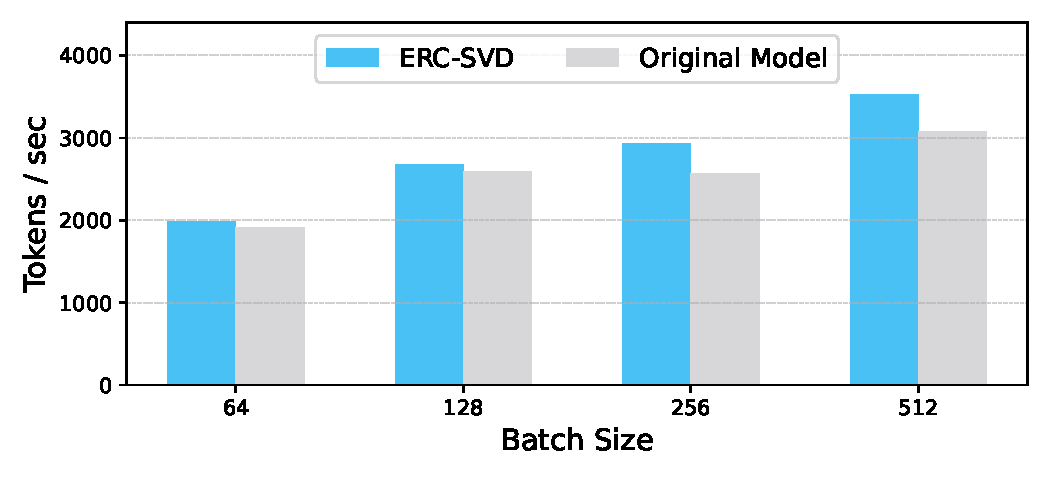
\includegraphics[width=\linewidth]{CPAL-2025-template/a_figures/throughput_comparison.pdf}
    \captionof{figure}{Throughput of LLaMA-7B and its 40\% compressed versions. The sequence length is 32.}
    \label{throughput_comparison}
  \end{minipage}%
  \hfill
  \begin{minipage}[t]{0.6\textwidth}
    \vspace{0pt}
    \centering

    \begin{subfigure}[t]{0.48\textwidth}
      \centering
      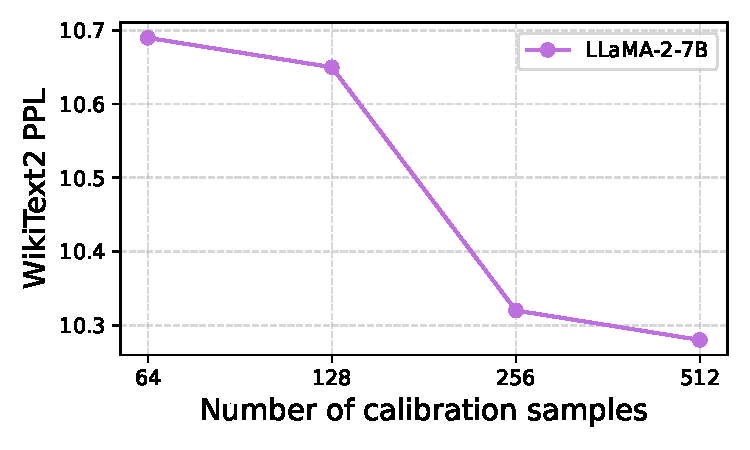
\includegraphics[width=\linewidth]{CPAL-2025-template/a_figures/different_samples_ppl.pdf}
    \end{subfigure}
    \hfill
    \begin{subfigure}[t]{0.48\textwidth}
      \centering
      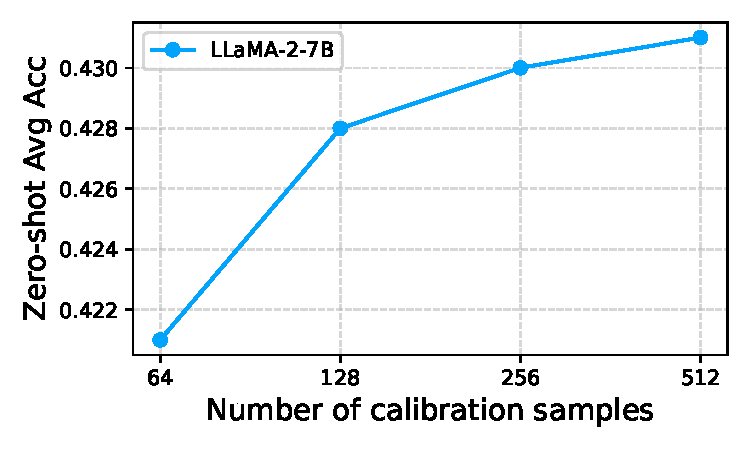
\includegraphics[width=\linewidth]{CPAL-2025-template/a_figures/different_samples_acc.pdf}
    \end{subfigure}

    \captionof{figure}{Impact of the number of calibration data samples on LLaMA-2-7B under 30\% compression ratio. (Left) Perplexity (\textcolor{blue}{$\downarrow$}). (Right) Average accuracy (\textcolor{green!60!black}{$\uparrow$}).}
    \label{calibration_samples_summary}
  \end{minipage}

\end{figure}

\subsection{Comparison with Smaller-Scale LLM} \label{gemma}
To further assess the effectiveness of ERC-SVD under relatively high compression ratios, we conduct a comparative evaluation of 50\% and 60\% compressed LLaMA-2-7B against Gemma-2-2B~\cite{gemma_2024}. Table~\ref{compare_gemma} presents the performance comparison between the compressed LLaMA-2-7B models and Gemma-2-2B. Under 50\% compression ratio (approximately 3.5B parameters), LLaMA-2-7B consistently outperforms Gemma-2-2B across most benchmarks. 
Even under a more aggressive 60\% compression ratio (around 2.8B parameters), the compressed model maintains competitive performance, remaining comparable to Gemma-2-2B. 


\begin{table}[t]
\centering
\caption{Performance comparison of Gemma-2-2B and LLaMA-2-7B compressed by ERC-SVD under 50\% and 60\% compression ratios (``\textsc{Ratio}'').}
\label{compare_gemma}
% \vspace{1mm}
% \vspace{-5pt}
\small
\resizebox{\textwidth}{!}{
\begin{tabular}{c|cc|ccc|cccccccc}
    \toprule
     \textsc{Model} & \textsc{Ratio} & \textbf{\#Params} & WikiText-2\textcolor{blue}{$\downarrow$} & PTB\textcolor{blue}{$\downarrow$} & C4\textcolor{blue}{$\downarrow$} & Openb.$\uparrow$  & ARC\_e$\uparrow$ & WinoG.$\uparrow$ & HellaS.$\uparrow$ & ARC\_c$\uparrow$ & PIQA$\uparrow$ & MathQA$\uparrow$ & Average\textcolor{green!60!black}{$\uparrow$}\\   
    \midrule
    \multirow{1}{*}{Gemma-2-2B}
                               & \cellcolor{white} - & \cellcolor{white} 3B & \cellcolor{white} 67.78 & \cellcolor{white} 374.60 & \cellcolor{white} 70.78 & \cellcolor{white} 0.13 & \cellcolor{white} 0.39 & \cellcolor{white} 0.51 & \cellcolor{white} 0.31 & \cellcolor{white} 0.19 & \cellcolor{white} 0.60 & \cellcolor{white} 0.23 & \cellcolor{white} 0.33 \\
    \midrule
    \multirow{2}{*}{LLaMA-2-7B}
                               & \cellcolor{cyan!10} 50\% & \cellcolor{cyan!10} 3.5B & \cellcolor{cyan!10} 24.26 & \cellcolor{cyan!10} 286.24 & \cellcolor{cyan!10} 100.34 & \cellcolor{cyan!10} 0.14 & \cellcolor{cyan!10} 0.35 & \cellcolor{cyan!10} 0.55 & \cellcolor{cyan!10} 0.31 & \cellcolor{cyan!10} 0.22 & \cellcolor{cyan!10} 0.59 & \cellcolor{cyan!10} 0.22 & \cellcolor{cyan!10} 0.34 \\
    \cmidrule{2-14}
                               & \cellcolor{cyan!10} 60\% & \cellcolor{cyan!10} 2.8B & \cellcolor{cyan!10} 68.59 & \cellcolor{cyan!10} 991.48 & \cellcolor{cyan!10} 255.70 & \cellcolor{cyan!10} 0.13 & \cellcolor{cyan!10} 0.29 & \cellcolor{cyan!10} 0.52 & \cellcolor{cyan!10} 0.28 & \cellcolor{cyan!10} 0.21 & \cellcolor{cyan!10} 0.55 & \cellcolor{cyan!10} 0.22 & \cellcolor{cyan!10} 0.31 \\
    \bottomrule
\end{tabular}
}
\end{table}
\vspace{-5pt}
\begin{table}[ht]
\centering
\caption{Performance (measured by accuracy (\textcolor{green!60!black}{$\uparrow$})) of original LLaVA-1.5-7B, and its 20\% compressed versions by SVD-LLM and ERC-SVD on VLM benchmarks. The best results are marked in \textbf{bold}.}
% \vspace{-5pt}
\label{some_benchmark}
\small
\resizebox{\textwidth}{!}{
\begin{tabular}{cc|ccccc}
    \toprule
     \textsc{Compression Ratio} & \textsc{Method} & POPE-random\textcolor{green!60!black}{$\uparrow$} & POPE-popular\textcolor{green!60!black}{$\uparrow$} & POPE-adversial\textcolor{green!60!black}{$\uparrow$} & TextVQA\textcolor{green!60!black}{$\uparrow$} & ScienceQA\textcolor{green!60!black}{$\uparrow$}\\
    \midrule
                            \textcolor{gray}{-}  & \cellcolor{white} \textcolor{gray}{Original} & \cellcolor{white} \textcolor{gray}{88.2} & \cellcolor{white} \textcolor{gray}{87.3} & \cellcolor{white} \textcolor{gray}{85.1} & \cellcolor{white} \textcolor{gray}{58.17} & \cellcolor{white} \textcolor{gray}{70.15}\\
    \midrule
    \multirow{2}{*}{20\%}      & \cellcolor{white} SVD-LLM & \cellcolor{white} 82.5 & \cellcolor{white} 83.2 & \cellcolor{white} 77.8 & \cellcolor{white} 30.68 & \cellcolor{white} 49.54\\
                               & \cellcolor{cyan!10} \textbf{ERC-SVD} & \cellcolor{cyan!10} \textbf{90.2} (\textcolor{green!60!black}{$\uparrow$9\%}) & \cellcolor{cyan!10} \textbf{87.7} (\textcolor{green!60!black}{$\uparrow$5\%}) & \cellcolor{cyan!10} \textbf{83.1} (\textcolor{green!60!black}{$\uparrow$7\%}) & \cellcolor{cyan!10} \textbf{50.86} (\textcolor{green!60!black}{$\uparrow$66\%}) & \cellcolor{cyan!10} \textbf{69.54} (\textcolor{green!60!black}{$\uparrow$40\%})\\
    \bottomrule
\end{tabular}
}
\end{table}


\subsection{Comparison with Pruning} \label{pruning}
Table~\ref{pruning_comparision} shows the performance of LLaMA-2-7B compressed by LLM-Pruner~\cite{ma2023llm} and ERC-SVD under different compression ratios on the WikiText-2 dataset. It can be observed that ERC-SVD consistently outperforms the pruning method, achieving a perplexity of 58.88 under 60\% compression ratio, compared to 114.23 for LLM-Pruner.

\subsection{Computation Complexity} \label{inference_efficiency_analysis}
ERC-SVD decomposes the original weight matrix $\boldsymbol{W}\in\mathbb{R}^{m\times n}$ into two low-rank matrices: $\hat{\boldsymbol{U}}_r\in\mathbb{R}^{m\times r}$ and $\hat{\boldsymbol{V}}_r\in\mathbb{R}^{r\times n}$. 
The layer compression ratio $R_l$ is computed as $R_l = 1 - \frac{(m+n)r}{mn}$. 
Under a fixed overall compression ratio $R_o$, the relationship between $R_l$ and $R_o$ is given by $R_l = \frac{N R_o}{k}$, where $N$ is the total number of layers and $k$ denotes the number of last layers to be compressed.

Given an input activation $\boldsymbol{X} \in \mathbb{R}^{n \times m}$, the original output is computed as $\boldsymbol{Y} = \boldsymbol{W} \boldsymbol{X}$. 
In the compressed model layer, an intermediate state is first computed as $\boldsymbol{I} = \hat{\boldsymbol{V}}_r \boldsymbol{X}$, followed by $\boldsymbol{Y} = \hat{\boldsymbol{U}}_r \boldsymbol{I}$.
The computational complexity of the original model is $N \cdot \mathcal{O}(m^2 n)$.
For the compressed model, the first $(N - k)$ layers remain uncompressed and retain a complexity of $(N - k) \cdot \mathcal{O}(m^2 n)$, while the compressed $k$ layers incur a cost of $k \cdot \mathcal{O}(m^2 r + r n m)$.
Thus, the total complexity becomes:
\begin{align}
    (N-k)\cdot\mathcal{O}(m^2n)+k\cdot\mathcal{O}(m^2r+rnm).
    \label{complexity}
\end{align}
And the rank $r$ is given by:
\begin{align}
    r = \frac{mn(1-R_l)}{m+n} = \frac{mn(k-NR_o)}{k(m+n)}.
    \label{rank}
\end{align}
Substituting the expression for $r$ into Equation~\ref{complexity}, we obtain the simplified total complexity:
\begin{align}
    \boxed{N(1-R_o)\cdot\mathcal{O}(m^2n)}
\end{align}
Compared to the original computation complexity $N \cdot \mathcal{O}(m^2 n)$. This indicates that the total computation cost is reduced proportionally to the overall compression ratio.
For example, if $R_o = 40$\%, the compressed model requires only 60\% of the original computational cost.

\subsection{Demonstration of Generated Contents} \label{generated_content}
Table~\ref{tab:zero_shot_text} shows the generation contents of models compressed by ERC-SVD compared to the original model under zero-shot conditions. The results indicate that across various input questions, compressed models consistently produce fluent, coherent, and highly relevant responses. Even at 40\% compression ratio, the compressed model can also deliver accurate and relevant answers to common sense questions. These results highlight the effectiveness of ERC-SVD.

\begin{table}[ht]
\centering
\caption{Generated contents of LLaMA-7B~\cite{touvron2023llama} compressed by ERC-SVD.}
\vspace{1mm}
\label{tab:zero_shot_text}
\renewcommand{\arraystretch}{1.3}
\setlength{\tabcolsep}{6pt}
\small

\resizebox{0.84\textwidth}{!}{
% \begin{tabular}{@{} >{\raggedright\arraybackslash}p{5cm} | c | >{\raggedright\arraybackslash}p{8cm} @{}}
\begin{tabular}{p{5cm}|c|p{8cm}}
\toprule
\textsc{Question} & \makecell{\textsc{Comp.}\\\textsc{Ratio}} & \textsc{Answer} \\
\midrule

\multirow{13}{=}{What is the responsibility of the AI assistant?}
& -   & The AI assistant is responsible for understanding the context and taking appropriate action. The AI assistant is responsible for understanding the intent, context, environment and taking appropriate actions. The AI assistant is responsible for interpreting. \\
\cmidrule{2-3}
& 20\% & The AI assistant should be responsible for providing an answer to questions. This means that when asked a question, you should do your best to answer it and not give any information other than what is requested. You should also consider the tone and intent. \\
\cmidrule{2-3}
& 30\% & The AI Assistant's job is to provide assistance to those who wish for assistance in their lives. It has no duty or obligation to assist those who do not desire assistance, nor does it have any duty to prevent. \\
\cmidrule{2-3}
& 40\% & The AI assistant does not have a specific role. The AI assistant will provide instructions to follow a path, and will give directions as an instruction to follow the path. \\
\midrule

\multirow{14}{=}{What is the universe? Explain this concept.}
& -   & The Universe is everything that exists. It includes all space, time, matter and energy. It also includes everything which has happened or will happen. The universe began about 13.7 billion years ago (the Big Bang) and will. \\
\cmidrule{2-3}
& 20\% & The universe is the whole of space and time. It consists of all things in space and all things that happen, or have happened. There are many theories on how it began; there were theories that it had no beginning at all. \\
\cmidrule{2-3}
& 30\% & The universe consists of everything in it, including matter and objects, space, the cosmos or outer space, and the galaxy system, as well as other galaxies that make up the Universe. The universe has its own life cycle. \\
\cmidrule{2-3}
& 40\% & In the universe, life is very diverse and complex. The universe is made up of many different objects. These objects are divided into groups. Each group consists of different objects that have specific properties. This group contains the universe, which is large. \\
\midrule

\multirow{11}{=}{Why do cars need fuel to run?}
& -   & Fuel is the lifeblood of a car. Without it, there's nothing to power
  the pistons and no way to drive. A car needs a constant supply of fuel. \\
\cmidrule{2-3}
& 20\% &  The fuel in the tank is burned to produce heat, which produces steam that drives a turbine, which turns a crankshaft. The crankshaft turns the wheels of the car, propelling it forward. \\
\cmidrule{2-3}
& 30\% & The fuel is the fuel in a car and it burns and goes up and up. It's important because it burns the gasoline, which makes it go faster. It's important because you can get energy out. \\
\cmidrule{2-3}
& 40\% & The fuel gives energy for the cars. The gasoline is used by a motor, which produces heat and air, heating up the engine. This allows the engines to travel faster, allowing them to reach higher speed. \\
\midrule

\multirow{9}{=}{Why do people feel hungry after exercise?}
& -   &  The answer is because the body burns more calories when you are exercising. You may not realize that the body uses up energy to digest food and absorb nutrients from it.  \\
\cmidrule{2-3}
& 20\% &  Because the body is more efficient at converting food into energy when inactive, so when active it needs to convert food into energy faster. This is why people often get hungry after exercise. \\
\cmidrule{2-3}
& 30\% & The reason people feel hungry after an activity is because they burn energy and energy is metabolised in the body.  \\
\cmidrule{2-3}
& 40\% & The reason the body is hungry after a long athletic activity was discovered by scientists in 1976. \\
\bottomrule

\end{tabular}
}
\end{table}

\subsection{ERC-SVD on Vision-Language Model}\label{ressvd:vlm}
In this section, we apply ERC-SVD to the language part of vision-language models (VLMs) such as LLaVA~\cite{liu2024improved}, and evaluate both quantitative and qualitative performance.

\subsubsection{Quantitative Results} \label{sec:benchmark}
We compare the performance of LLaVA-1.5-7B~\cite{liu2024improved} compressed using SVD-LLM~\cite{wang2024svd} and ERC-SVD under 20\% compression ratio. 
We report results on several benchmarks: POPE~\cite{li2023evaluating}, TextVQA~\cite{singh2019towards}, and ScienceQA~\cite{lu2022learn}.
The results, shown in Table~\ref{some_benchmark}, indicate that ERC-SVD consistently outperforms SVD-LLM across all benchmarks. 
Notably, it achieves substantial relative improvements, 66\% on TextVQA and 40\% on ScienceQA.
Moreover, on the POPE-random and POPE-popular subsets, the model compressed by ERC-SVD even surpasses the original LLaVA-1.5-7B.

\subsubsection{Qualitative Results} \label{sec:qualitative}
As shown in Figure~\ref{fig:image_captioning}, LLaVA-1.5-7B compressed with ERC-SVD under 20\% compression ratio is still able to produce image captions that are faithful to the visual content.
This indicates that the model retains its ability to interpret and describe images accurately, despite parameter reduction. 
\begin{figure}[h]
  \centering
  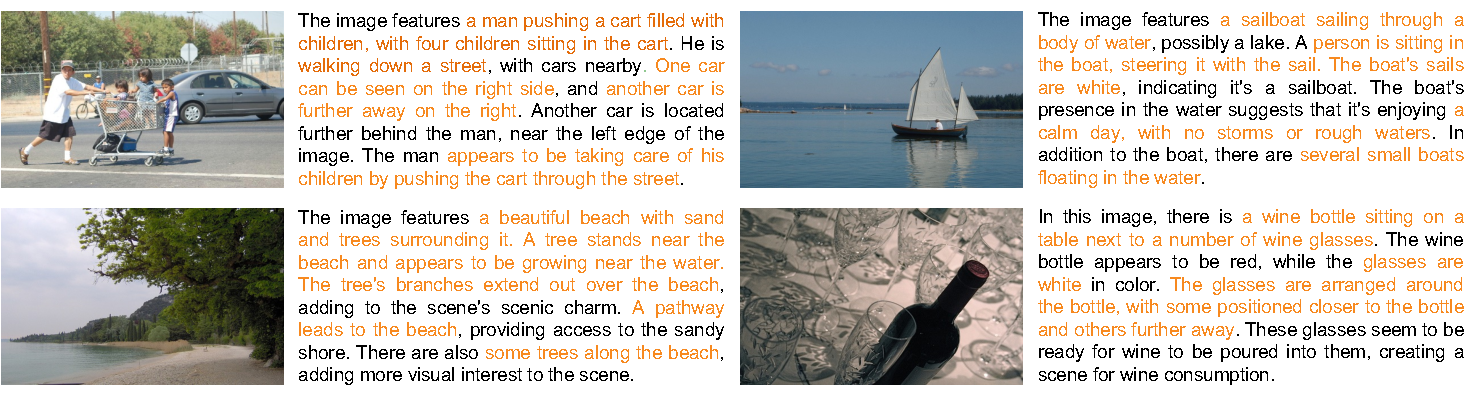
\includegraphics[width=\linewidth]{CPAL-2025-template/a_figures/image_caption.pdf} 
  \caption{Image captioning results of LLaVA-1.5-7B compressed by ERC-SVD under 20\% compression ratio. Captions that accurately describe the image content are highlighted in \textcolor{lightergreen}{orange}.}
  \label{fig:image_captioning}
\end{figure}

Figure~\ref{fig:vqa} presents the visual question answering results of LLaVA-1.5-7B compressed by ERC-SVD.
The model retains strong performance across these question types, indicating that its multi-modal reasoning capability remains intact despite the compression.
\begin{figure}[H]
  \centering
  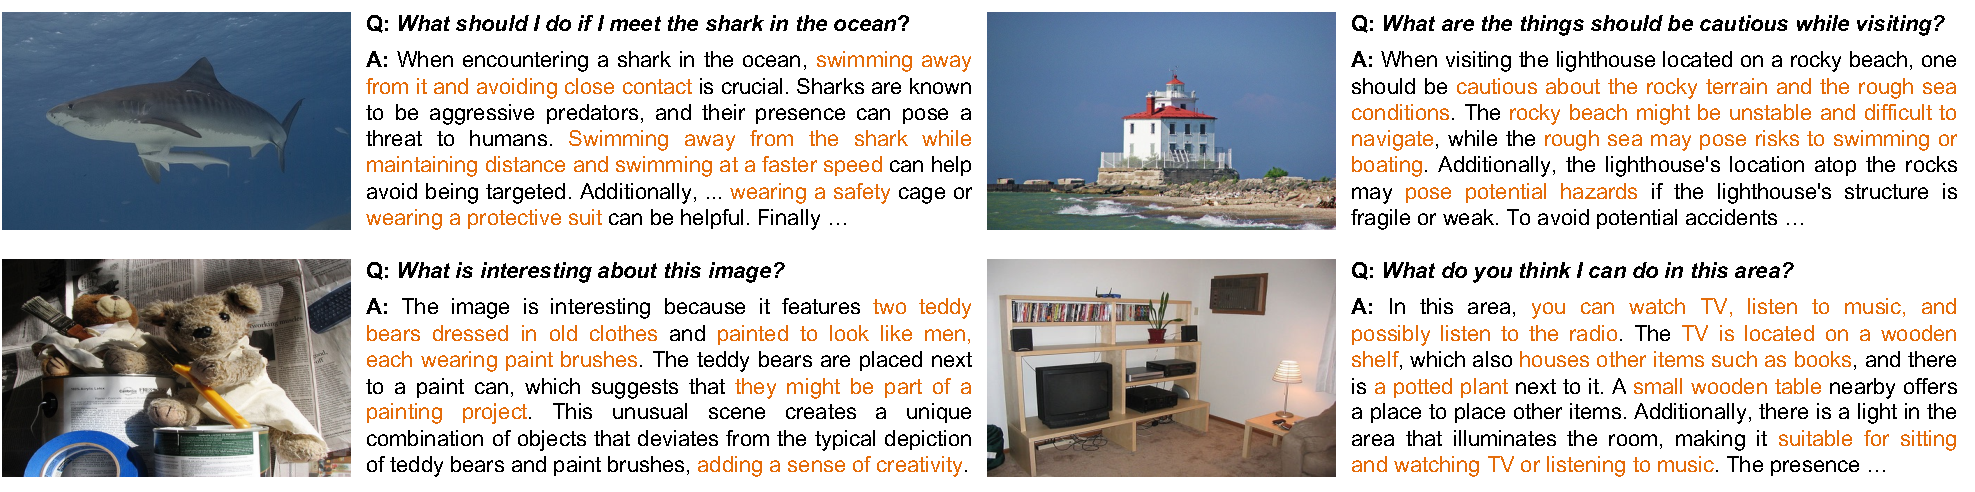
\includegraphics[width=\linewidth]{CPAL-2025-template/a_figures/vqa.pdf} 
  \caption{Visual question answering outputs generated by LLaVA-1.5-7B compressed using ERC-SVD under 20\% compression ratio. Questions (Q) and model answers (A) are provided, correct answers are highlighted in \textcolor{lightergreen}{orange} to emphasize answer quality retention.}
  \label{fig:vqa}
\end{figure}


\subsection{Future Work}
While this work focuses on general LLM compression, the low-rank structures identified via SVD hold significant potential for reasoning LLMs~\cite{jaech2024openai,yang2025qwen3,feng2025efficient}. Beyond autoregressive language tasks, the principles of SVD-based compression are readily transferable to diffusion frameworks~\cite{rombach2022high,zhu2025obs,bai2026dice}. In related tasks, the Transformer-based denoisers often exhibit extreme parameter redundancy. By leveraging ERC-SVD to decompose attention layers, maybe we can accelerate the iterative sampling process, making real-time deployment of generative models on edge devices more feasible without sacrificing structural fidelity. Furthermore, the intersection of model compression and hallucination mitigation~\cite{tonmoy2024comprehensive,zhang2025poison} presents an intriguing research frontier. We hypothesize that low-rank approximations could potentially filter out the noise that contributes to factually incorrect generations, a direction we intend to explore in future work.